\subsection{Precios}
\subsubsection{Análisis exploratorio}

Para el análisis de los precios se cuenta con un poco mas de 1.5 millones de registros, que indican el precio de cada producto e información de contexto. Por medio de otros set de datos, como ser el que tiene los datos de las sucursales y detalles de los productos que se harán análisis particulares en secciones próximas, pero en este caso el análisis estará apuntado al análisis de los precios.\\

Lo primero que se busca es por medio de un histograma conocer como es la distribución de los precios, como objetivo se busca entender si los mismos siguen algún patrón.\\


\begin{center}
    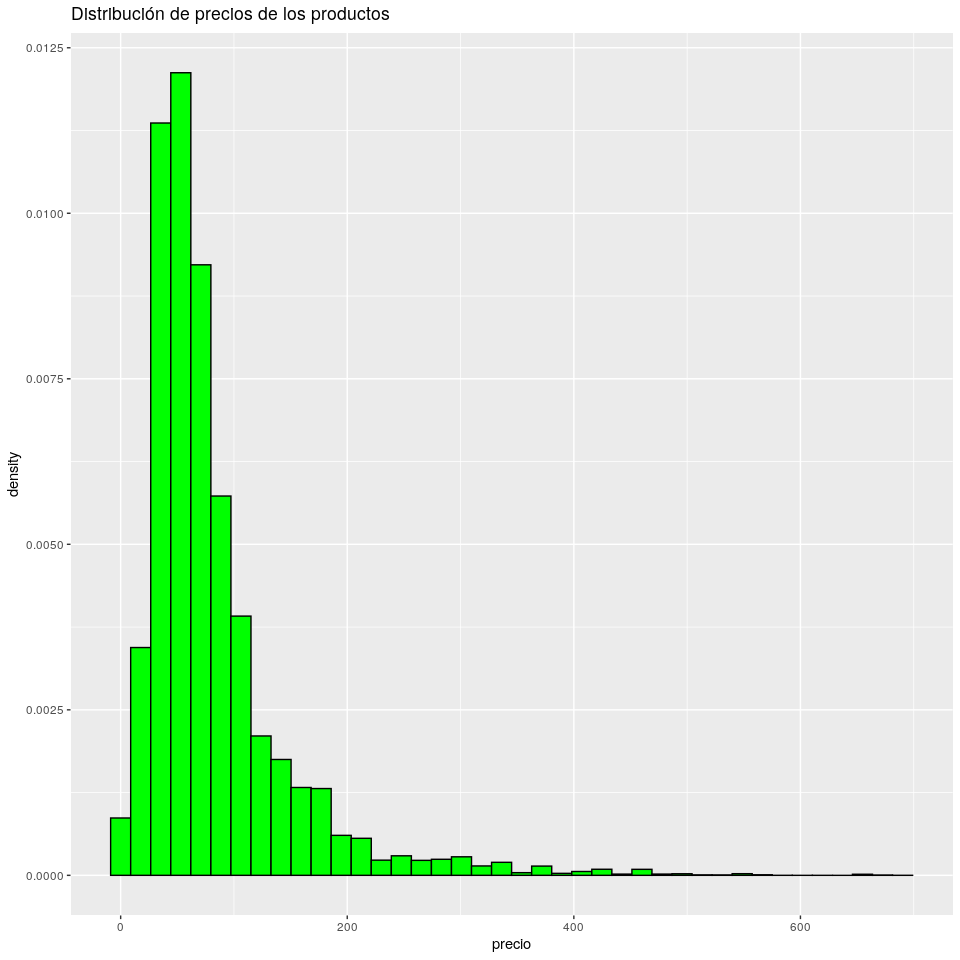
\includegraphics[scale=0.6]{img/histograma_precios_productos.png}
\end{center}

En cuanto al gráfico del histograma, se puede evidenciar claramente una asimetría a derecha y como primer
aproximación se puede ver como la mayoría de las mediciones marcan valores cercanos a los 80 Pesos.\\
Pasando en limpio, se visualiza en la siguiente tabla los valores significativos de todos los precios.\\

\begin{center}
 \begin{tabular}{||l c c c c c||} 
 \hline
 Minimo & 1st Qu & Mediana & Promedio & 3rd Qu & Máximo \\ [0.5ex] 
 \hline\hline
 2.85 & 42.00 & 62.90 & 80.79 & 95.99 & 693.00 \\ 
 \hline
 \hline
\end{tabular}
\end{center}

En principio el valor máximo y mínimo observado podrían indicar la presencia de valores anómalos o outliers en las mediciones, sobre todo teniendo en cuenta que el valor de mediana y Promedio es del orden de magnitud diferente a los dos extremos.


\subsubsection{Datos Atípicos}

Interesa conocer si la presencia de datos atípicos dentro de las mediciones de precios, estos podrían seguir dos naturalezas de origen:

\begin{enumerate}
    \item Datos mal cargados o originados con algún defecto en su medición.
    \item Precios que se corresponden con productos, pero que dependiendo de la cantidad de casos y de su naturaleza quizás no tenga sentidos mantenerlos en el análisis.
\end{enumerate}


Se generara un primer boxPlot para entender gráficamente como es la distribución de los precios para encontrar datos atípicos y poder catalogarlos y luego analizar si es necesario quitarlos o dejarlos entre los datos a estudiar.



\begin{center}
    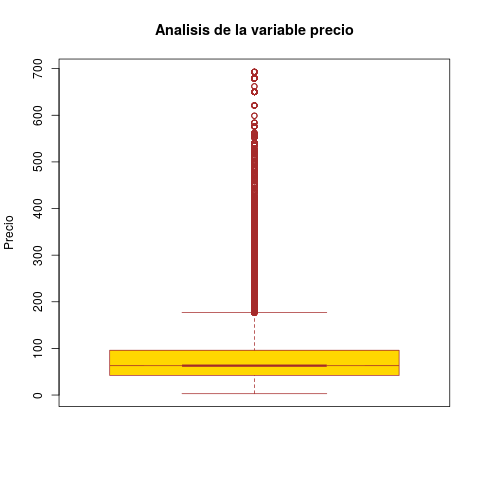
\includegraphics[scale=0.6]{img/boxplot_basico.png}
\end{center}




Cómo se observa datos que pueden considerarse outliers son aquellos precios observados con un valor mayor a \$200,00. \\
Como se puede evidenciar hay gran cantidad de datos por sobre el bigote superior, con lo cual se ensayaron algunas técnicas para exploración de estos datos, para entender si eran o no datos atípicos.\\
En un primer momento se realizo el mismo BoxPlot pero eliminando toda medición ubicada a 1,5 veces la distancia inercuartil por arriba y por abajo, como resultado se obtuvo un diagrama muy similar al anterior donde la diferencia radicaba que los outliers se empezaban a producir del mismo modo a partir de los \$150 con lo cual no significo en ningún mejora para el análisis.\\
En segundo lugar lo que se propuso eliminar un porcentaje de datos en las puntas superiores e inferiores pero nuevamente no mostraron resultados concluyentes.\\
Fue por ello y debido a que la mayor cantidad de datos atípicos se mostraban en las bandas mas altas de precios que se decidido realizar un análisis de BoxPlot pero con los valores superiores a \$290 para entender como era la distribución de esos valores altos en mas detalle.


\begin{center}
    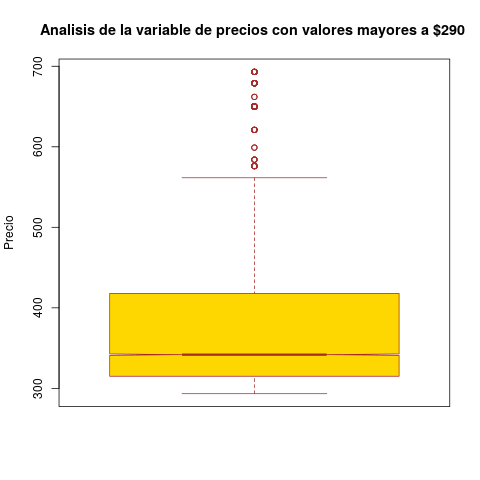
\includegraphics[scale=0.6]{img/boxplot_mayor290.png}
\end{center}

Se aprecia que existen muy pocas observaciones ahora por encima del bigote superior por lo que se llevo a cabo una investigación de estas mediciones una a una para entender cual era el origen de las mismas.\\
Lo que se encontró en estos casos, es que estas mediciones se correspondían con precios correctamente medidos pero sobre productos de alto valor como ser una bebida importada (Whiskey) o similar, no representando un error en la medición ni tampoco un conjunto de datos aislados, sino pequeños grupos que representan un producto en particular y que en todas sus mediciones se comportan de manera similar.\\
Es por ello que si bien, existen desigualdades entre los precios, se decide no eliminar partes ni recortar el set original de datos.







\subsection{Barrios Porteños}
\subsubsection{Análisis exploratorio}

Ya que se contaba con el dato de latitud y longitud donde cada punto de venta estaba ubicado, se comenzó el análisis de los datos haciendo un mapeo entre la posición geoespacial de cada punto de venta y los polígonos que describen a cada barrio, de modo de poder determinar para cada punto de venta a que barrio pertenecía, lo que se busca conocer con este análisis es entender si los puntos de venta están repartidos uniformemente en la ciudad y en caso contrario si esta distribución sigue alguna lógica. Con este primer estudio de las coordenadas de los puntos de ventas, se obtiene el siguiente mapa:


%\begin{center}
%    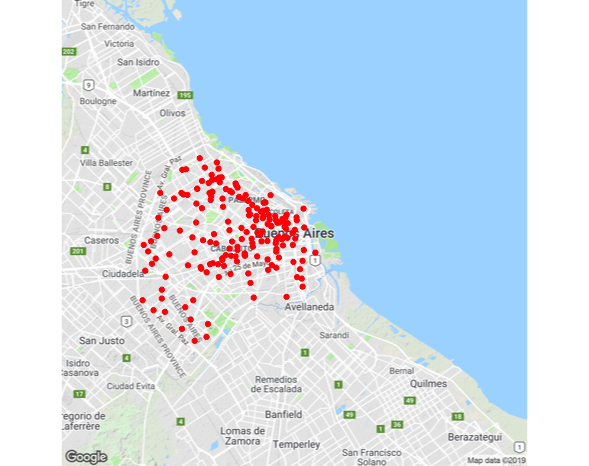
\includegraphics[scale=0.8]{img/mapa.png}
%\end{center}



\begin{figure}[h]
\makebox[\textwidth]{
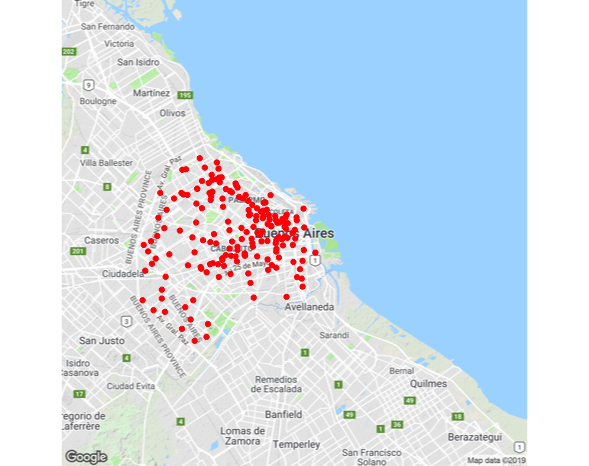
\includegraphics[width=0.4\paperwidth, height=0.4\paperheight, keepaspectratio]{img/mapa.png}
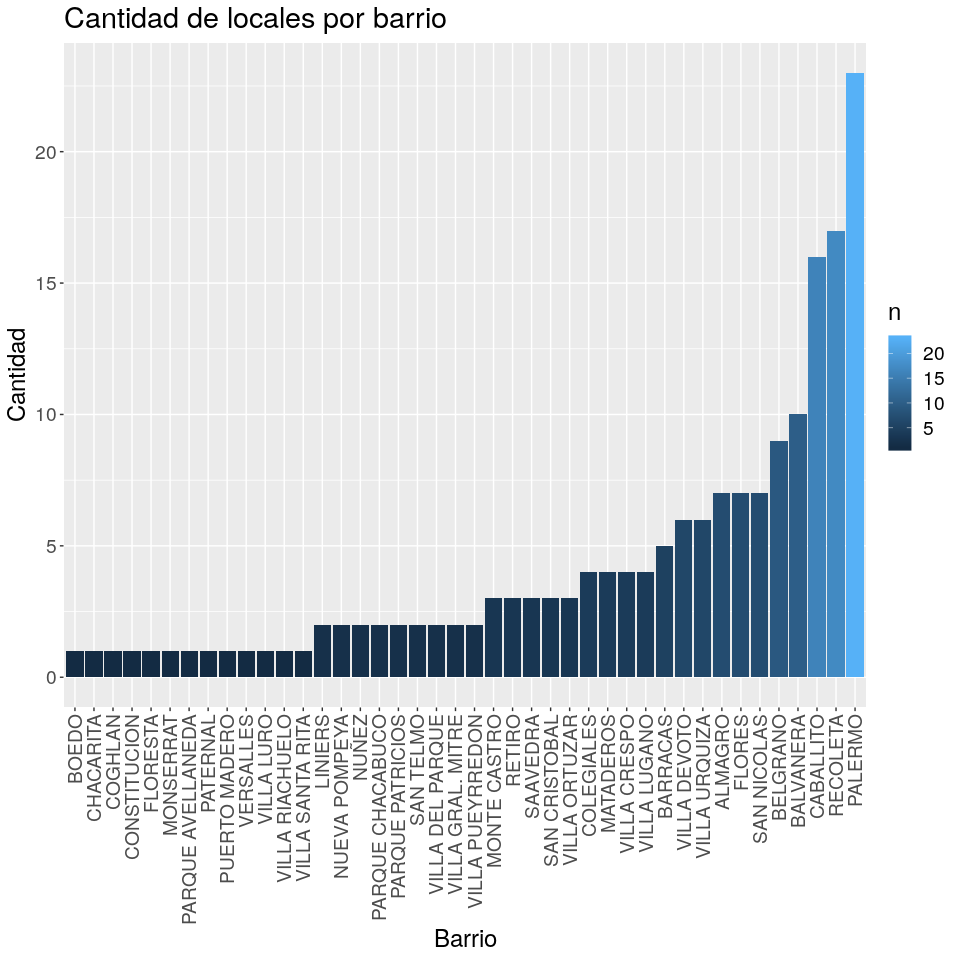
\includegraphics[width=0.4\paperwidth, height=0.4\paperheight, keepaspectratio]{img/cantLocales_vs_barrio.png}
}
\end{figure}


Lo que se puede observar de este primer análisis es que los puntos de venta no están repartidos uniformemente y se evidencia una mayor concentración de puntos de venta hacia la zona del centro porteño.\\
Por otro lado en el segundo gráfico se observa una asimetría a izquierda, teniendo 5 barrios de 42 el 44\% del total de las sucursales y solo PALERMO presenta el 13\% de las mismas.\\


Lo que se busca a continuación es entender como es el precio medio de los productos agrupados por barrio, esto ayudara a poder dilucidar si existe alguna correlación entre la cantidad de puntos de ventas en un barrio con su precio promedio.
Es necesariamente el barrio con menos cantidad de puntos de ventas el que tiene el precio mas alto promedio (por tener una menor cantidad de oferta)?\\
O por el contrario el mayor precio se da en barrios con mas cantidad de locales?


\begin{figure}[H]
\makebox[\textwidth]{
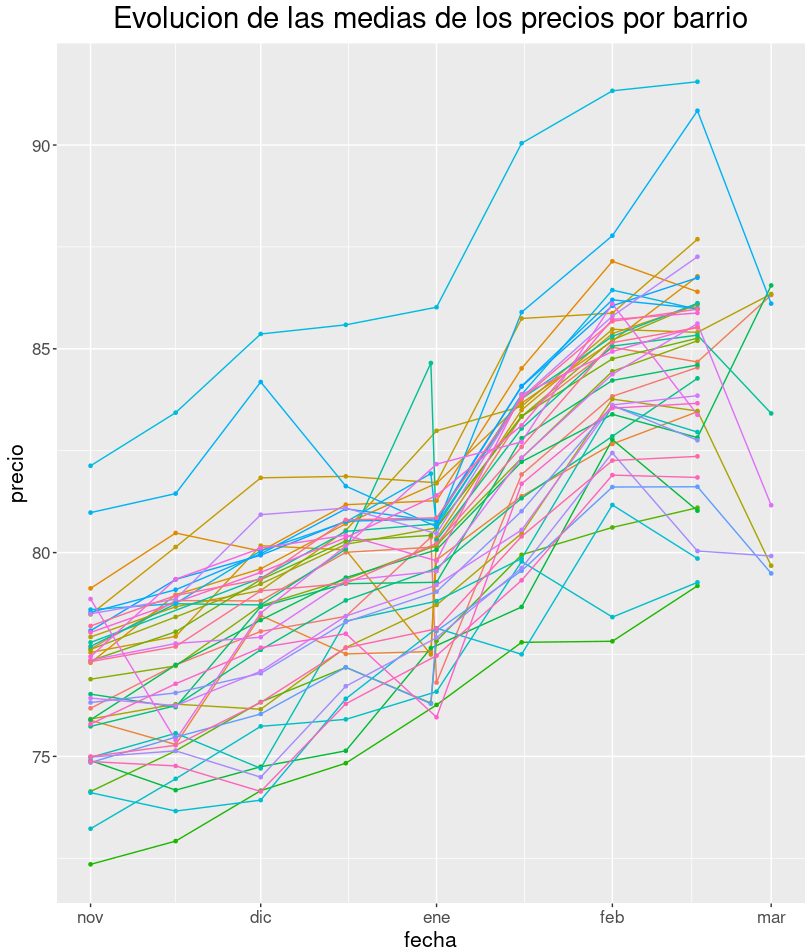
\includegraphics[width=0.4\paperwidth, height=0.4\paperheight, keepaspectratio]{img/mediaPrecios_agrupados_xBarrio.png}
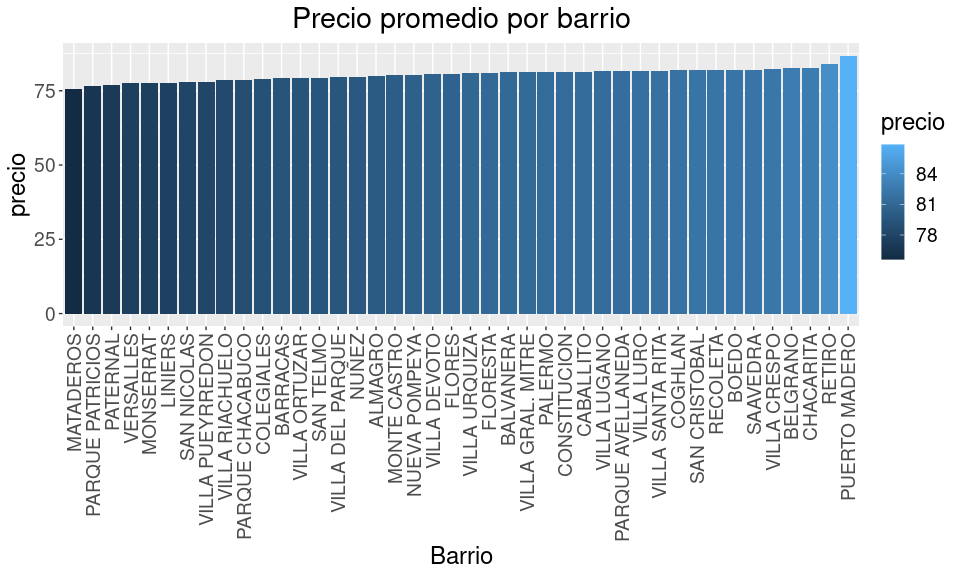
\includegraphics[width=0.4\paperwidth, height=0.4\paperheight, keepaspectratio]{img/mediaPrecios_xBarrio.png}
}
\end{figure}

Del análisis realizado sobre los distintos barrios de la Ciudad e Buenos Aires se pueden desprender dos conclusiones prematuramente, una es que si bien algunos barrios hay tenido diferencia de precios según el corte mayor o menor la tendencia en la ventana de tiempo estudiada es siempre al alza. La segunda es que Mataderos, el barrio con el promedio de precios mas bajos de entre los 42, tenia muchos mas puntos de venta que Puerto Madero sin embargo este ultimo tiene los mayores precios en promedio de entre todos los barrios porteños. Palermo quien ostenta tener el 13\%  de los puntos de venta de la ciudad queda en el puesto 17 de entre los 42 barrios en nivel de precio. Con lo cual hasta ahora no se puede afirmar que la cantidad de sucursales no son lo único que influye para determinar el precio promedio de los productos.

TODO: Considerar agregar el precio promedio por metro cuadrado en el análisis.



\subsection{Puntos de venta}
\subsubsection{Análisis exploratorio}

Llega el turno de entender como el tipo de punto de venta influye en la distribución de los mismos por la ciudad y en la formación de precios. Para eso, cabe aclarar que se tuvo en cuenta los dos tipos que están representados en nuestros datos el de $Supermercado$ y el de $Hipermercado$ siendo este ultimo por lo general de mayor tamaño y contar con mas cantidad de productos a la venta. Además del tamaño del punto de venta otro estudio que se realizará es el de bandera,  marca o razón social. Cabe destacar que algunas cadenas de supermercado tienen mas de una baderna, tema que se ira ahondando mas adelante.\\
Para comenzar algo que interesa conocer es de los 175 locales si la distribución de las banderas en esas sucursales es uniforme o si hay banderas que tienen predominancia sobre otras.

\begin{center}
    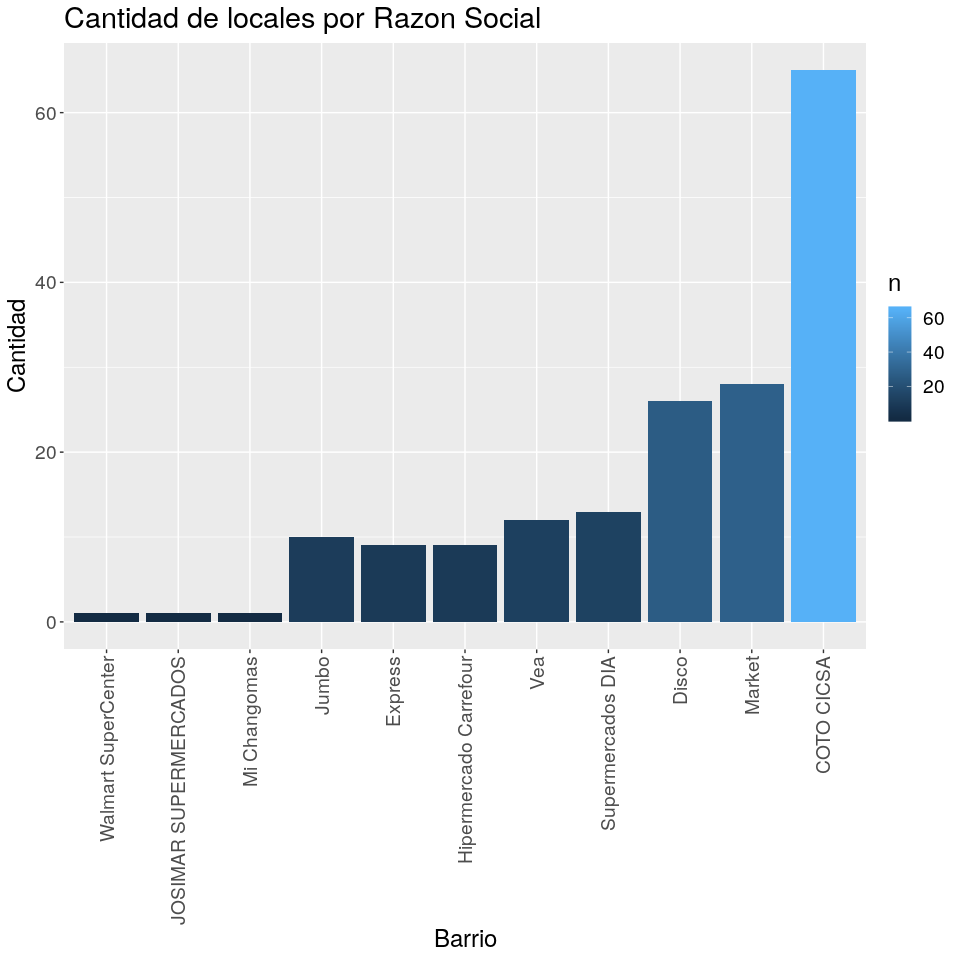
\includegraphics[scale=0.6]{img/cantLocales_vs_bandera.png}
\end{center}


\begin{center}
 \begin{tabular}{||l c||} 
 \hline
 Bandera & Cantidad \\ [0.5ex] 
 \hline\hline
 COTO CICSA & 65 \\ 
 \hline
 Market & 28 \\
 \hline
 Disco & 26 \\
 \hline
 Supermercados DIA & 13 \\
 \hline
 Vea & 12 \\
 \hline
 Jumbo & 10 \\
 \hline
 Express & 9 \\
 \hline
 Hipermercado Carrefour & 9 \\
 \hline
 JOSIMAR SUPERMERCADOS & 1 \\
 \hline
 Mi Changomas & 1 \\
 \hline
 Walmart SuperCenter & 1 \\[1ex]
 \hline
 \hline
\end{tabular}
\end{center}


Siempre teniendo en cuenta que se están mirando negocios de venta de productos del tipo súper o hiper, se resalta claramente que en la Ciudad de Buenos Aire, la bandera COTO CICSA una predominancia de casi el 40\% de los locales de venta.\\

Luego de haber tenido este análisis incipiente en la distribución de puntos de venta por las distintas banderas de las empresas, interesa conocer dada una bandera como es la distribución de los precios para todo el periodo estudiado, esto ayudará a entender si existe una bandera con alta predominancia de locales y son estos los que contienen los precios mas altos o mas bajos entonces se podría decir que como dicha bandera tiene una alta oferta de estos precios la misma podría entenderse como una formadora de precios.\\
\\



\begin{figure}[h]
\centering
\begin{subfigure}{.5\textwidth}
  \centering
  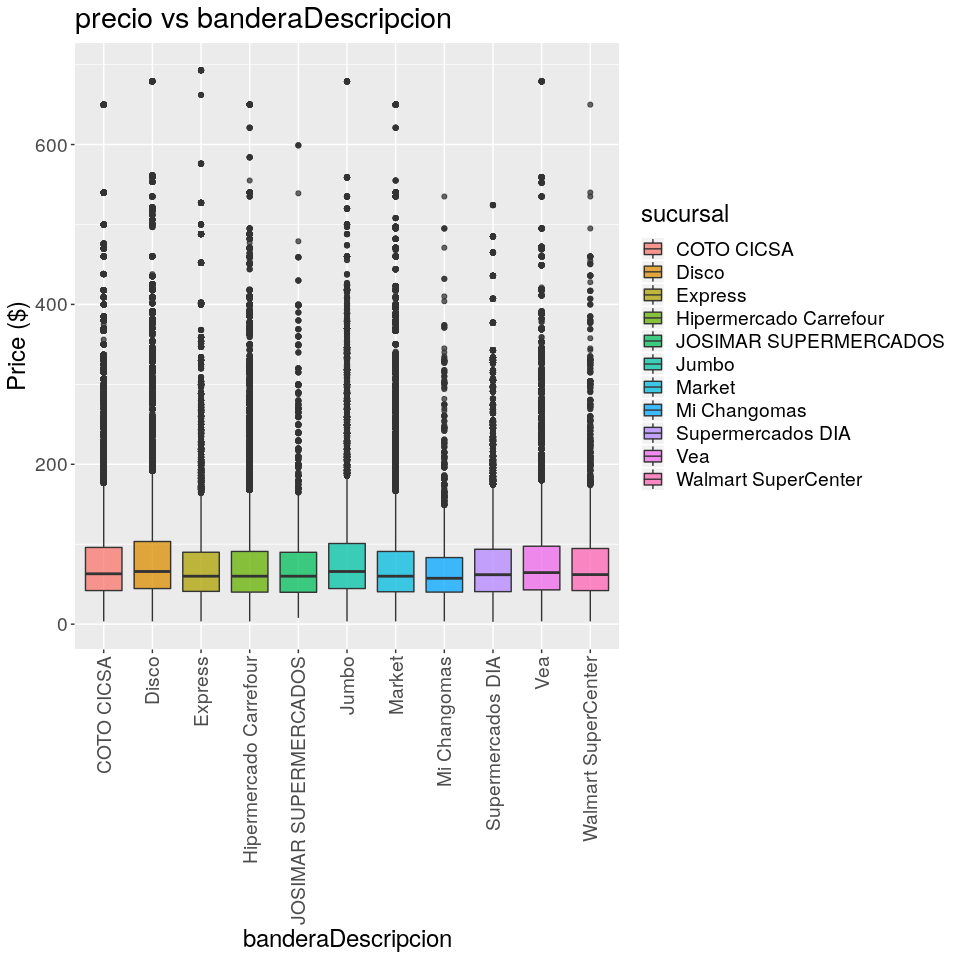
\includegraphics[width=0.4\paperwidth, height=0.4\paperheight, keepaspectratio]{img/precio_vs_bandera.png}
  %\caption{A subfigure}
  %\label{fig:sub1}
\end{subfigure}%
\begin{subfigure}{.5\textwidth}
  \centering
  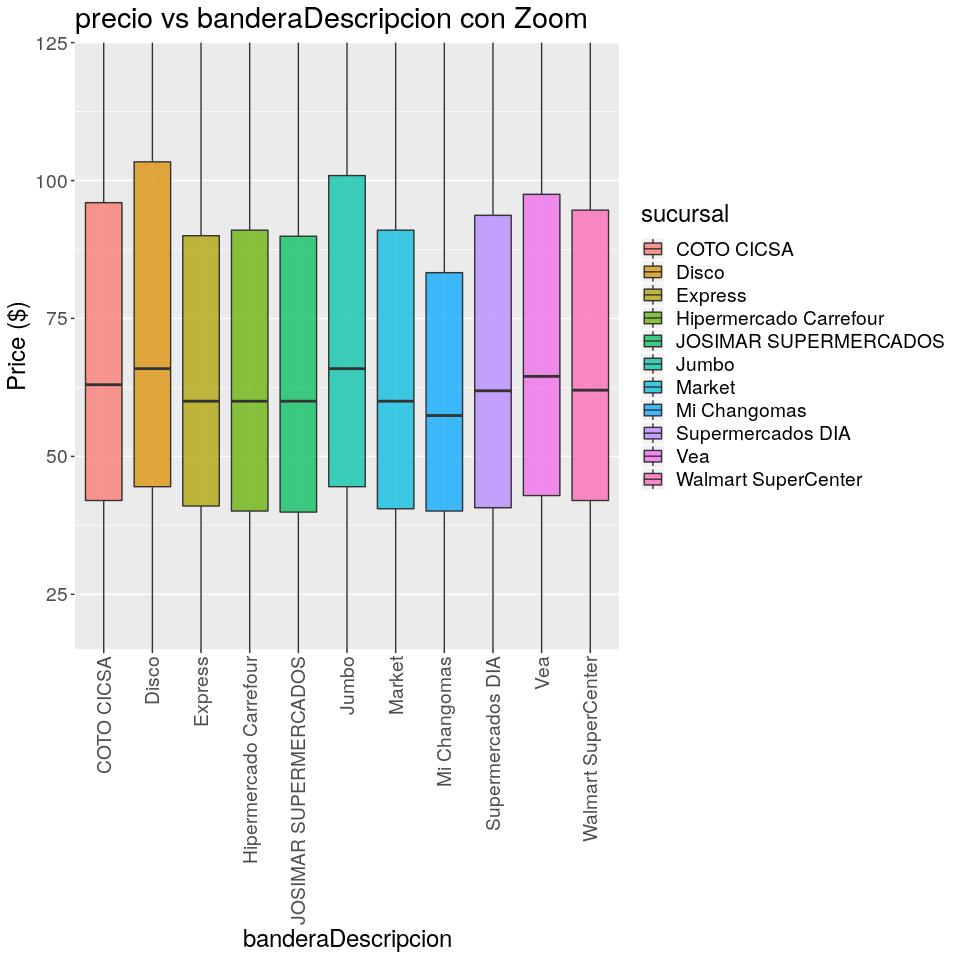
\includegraphics[width=0.4\paperwidth, height=0.4\paperheight, keepaspectratio]{img/precio_vs_bandera_zoom.png}
  %\caption{A subfigure}
  %\label{fig:sub2}
\end{subfigure}
\caption{Distribucion de precios en las distintas banderas}
\label{fig:test}
\end{figure}


Para hacer este análisis se utilizo BoxPlot, en el gráfico de la izquierda podemos ver como todas las banderas tienen datos de precios muy por arriba del limite superior de las cajas, la gran mayoría entre el rango de los 180 y los 420 PESOS. Sin embargo lo que es datos en limite inferior, ninguna bandera presenta ya que hay gran cantidad de productos con precios bajos.\\
En el gráfico de la derecha, lo que se obtiene es un zoom en la zona de las cajas, para entender como es la distribución de los cuantiles y la Mediana. Ahí claramente se puede ver que DISCO y JUMBO (ambos de la misma empresa) tienen los precios mas altos seguidos por VEA, también del mismo grupo, acaparando entre los 3 
48 puntos de venta de los 175 totales, en segundo lugar como grupo esta COTO CISCA con 65 puntos de venta de entre las 175.\\
Dado este análisis, se puede concluir que de las 175 sucursales estudiadas dos empresas (COTO y JUMBO-DISCO-VEA) acumulan casi el 65\% de la presencia en el mercado teniendo estos los precios mas altos de entre todas las banderas.\\


A continuación buscamos haciendo un corte cada 15 días para calcular el promedio de precios ver por grupo de banderas (JUMBO-DISCO-VEA juntos)

\begin{center}
    
\end{center}







\begin{figure}[h]
\centering
\begin{subfigure}{.5\textwidth}
  \centering
  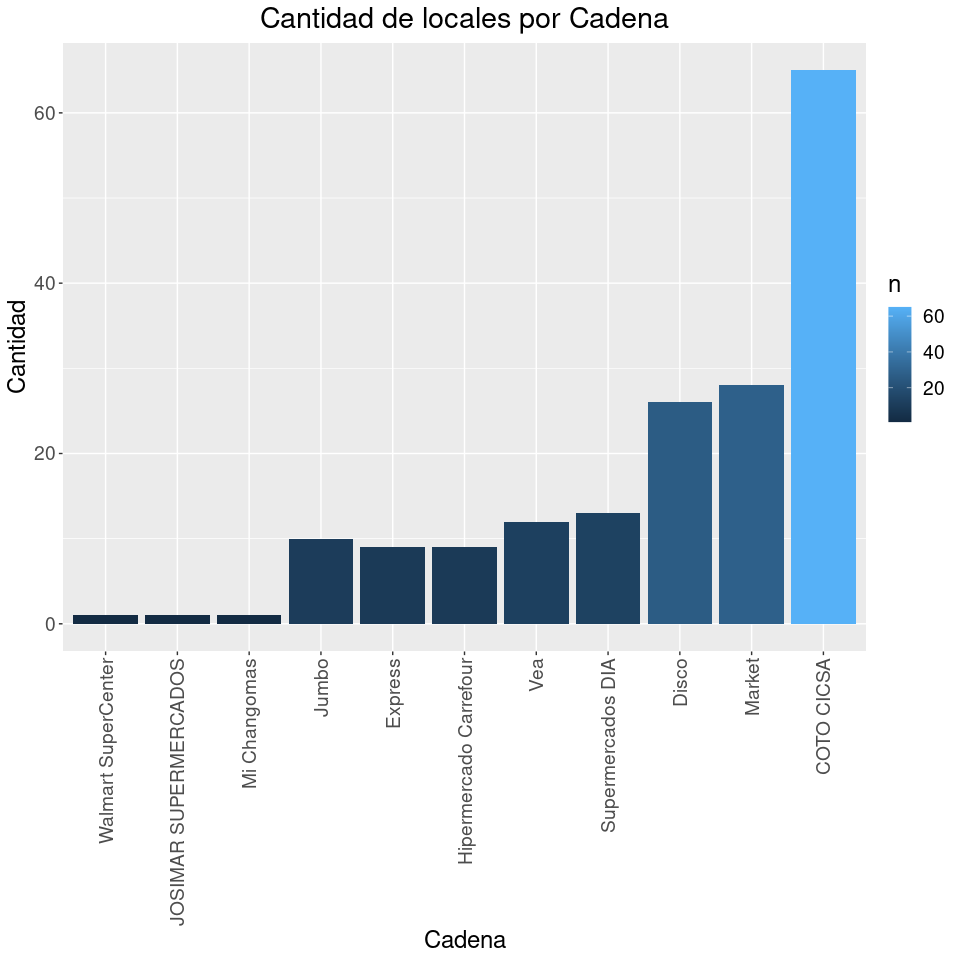
\includegraphics[width=0.6\paperwidth, height=0.4\paperheight, keepaspectratio]{img/mediaPrecios_vs_bandera.png}
  %\caption{A subfigure}
  %\label{fig:sub1}
\end{subfigure}%
\begin{subfigure}{.5\textwidth}
  \centering
  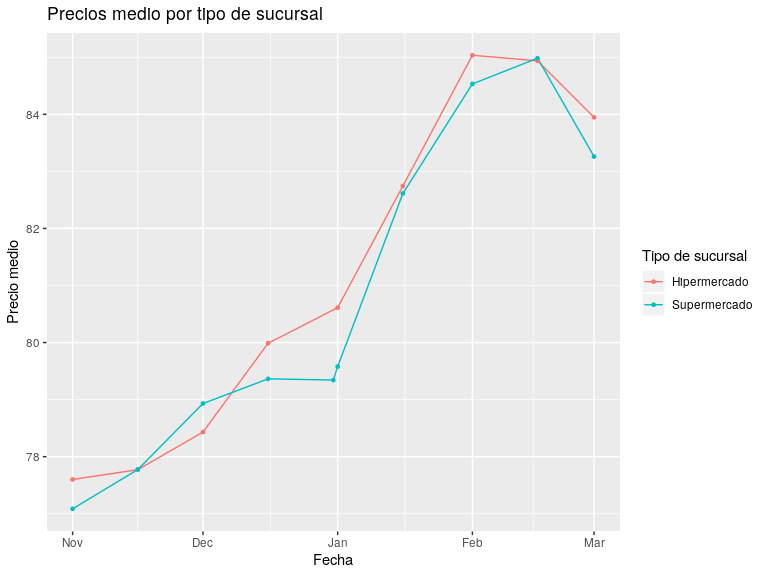
\includegraphics[width=0.5\paperwidth, height=0.4\paperheight, keepaspectratio]{img/mediaPrecios_vs_tipoLocal.png}
  %\caption{A subfigure}
  %\label{fig:sub2}
\end{subfigure}
\caption{Distribución de precios por tipo bandera y comparativa de promedios cada 15 dias}
\label{fig:test}
\end{figure}

Se puede comprobar en el gráfico de la izquierda que claramente con el corte promedio cada 15 días el conglomerado de Jumbo y Coto siguen una curva muy parecida y claramente tienen los precios promedio mas altos y además definen en el tiempo una tendencia al alza.\\
El resto de las banderas, con menor presencia también tienen una tendencia al alza pero con precios promedios menores.\\
En el gráfico de la derecha se observa una comparativa entre todas las banderas diferenciando los Supermercados de los Hipermercados. Si bien la tendencia y las curvas de evolución de los precios es muy similar, en la mayoría de los cortes los precios promedio en los Hipermercados es superior a los de los Supermercados.

